\section{Results}


\subsection{Low-dimensional data}

\subsubsection*{One-dimensional data}

\begin{figure}
  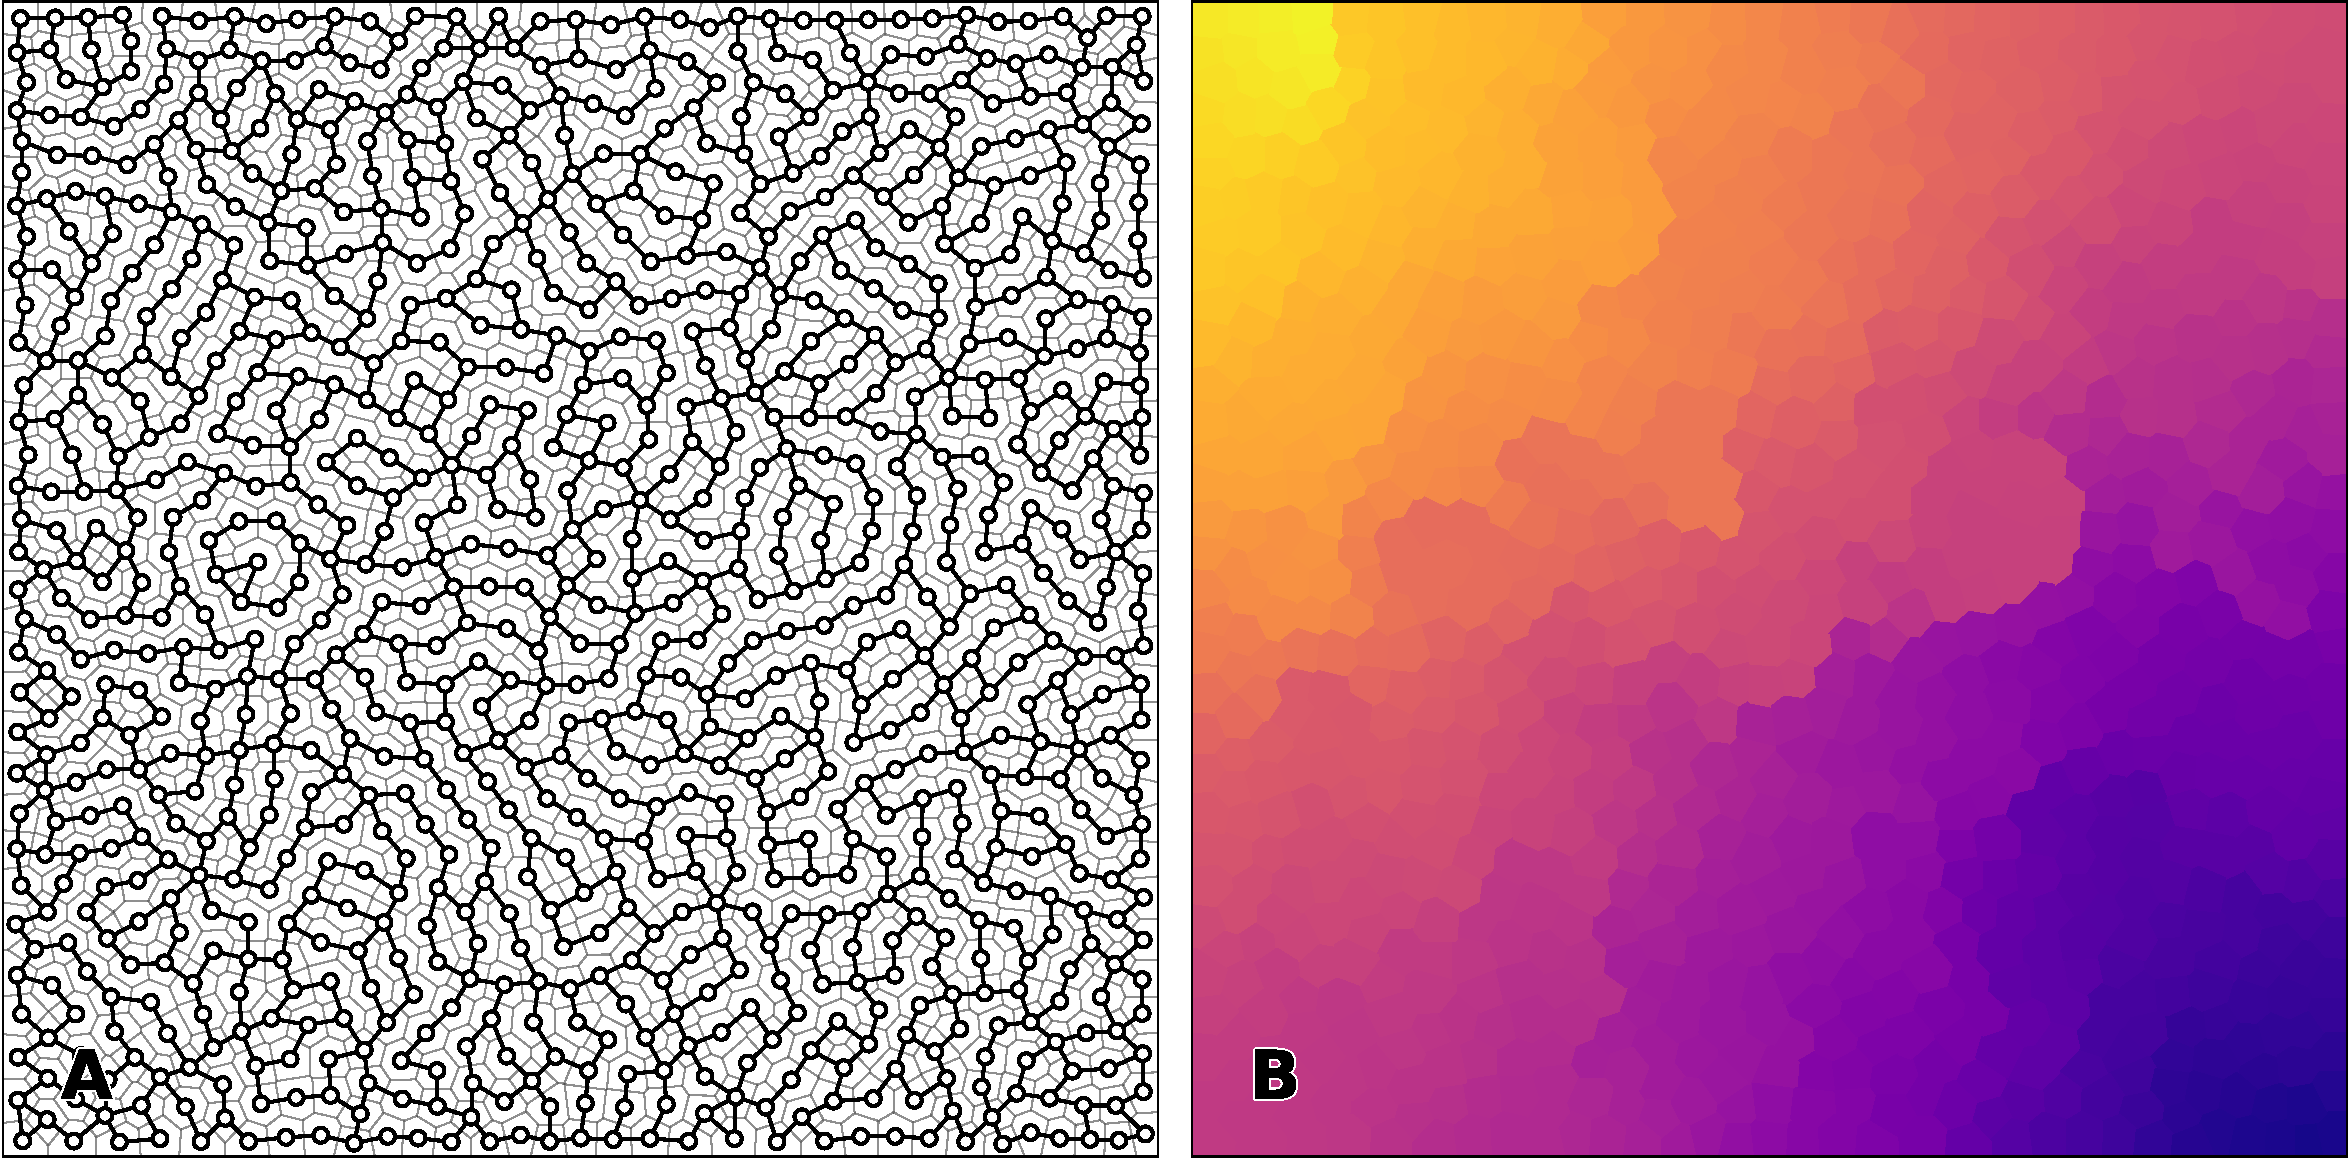
\includegraphics[width=\columnwidth]{figures/vsom-scalar-1.pdf}

  \vspace{2mm}
  
  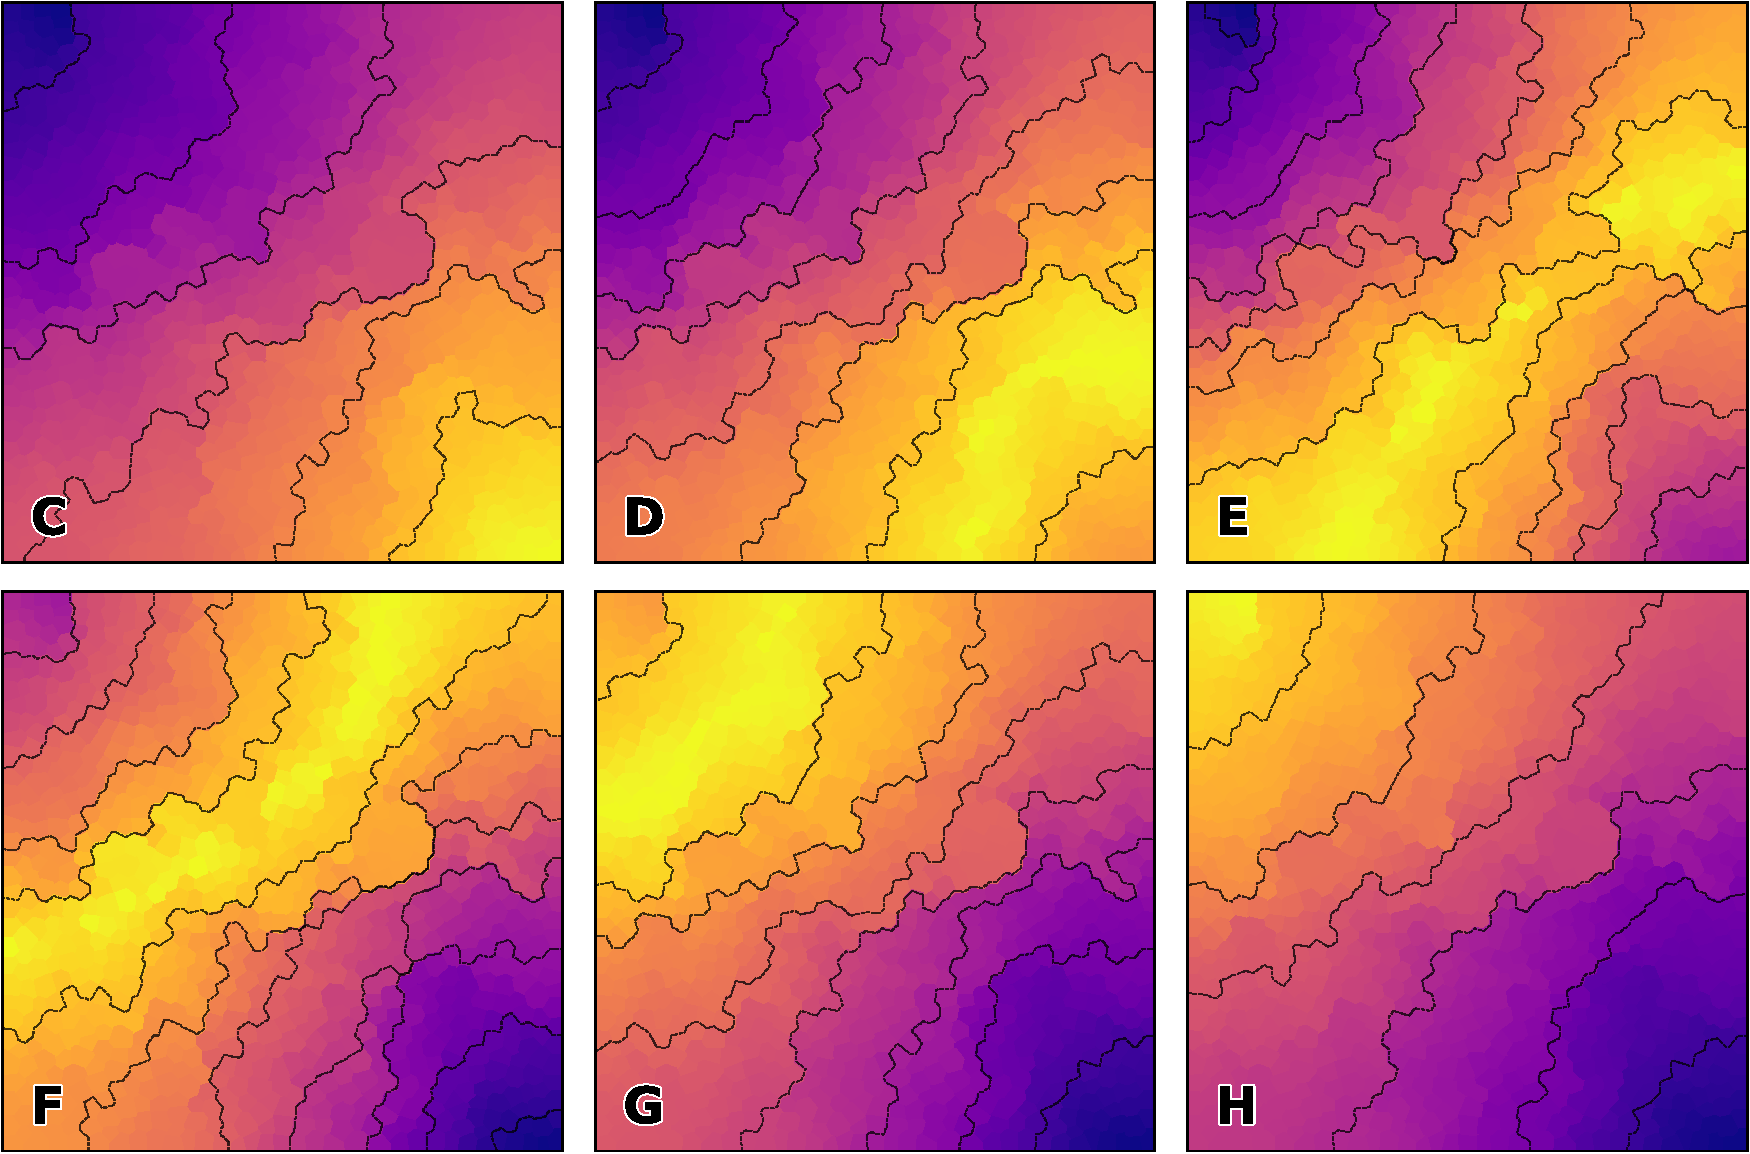
\includegraphics[width=\columnwidth]{figures/vsom-scalar-2.pdf}

  \vspace{2mm}
  
  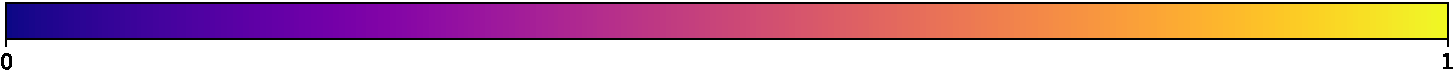
\includegraphics[width=\columnwidth]{figures/colormap.pdf}
  
  \caption{Voronoidal SOM made of 1003 neurons with a 2-nearest neighbors
    induced topology. Model has been trained for 10,000 epochs on random
    uniform scalars in [0,1]. \textbf{A} Map topology in the neural
    space. \textbf{B} Map prototypes displayed in neural space using Voronoi
    cells (whose color indicates prototype according to colormap). \textbf{C to
      H} Map activity for some random data (\textbf{C}:0.0, \textbf{D}:0.2,
    \textbf{E}: 0.4, \textbf{F}:0.6, \textbf{G}:0.8, \textbf{H}:1.0).}
\end{figure}

\begin{figure}
  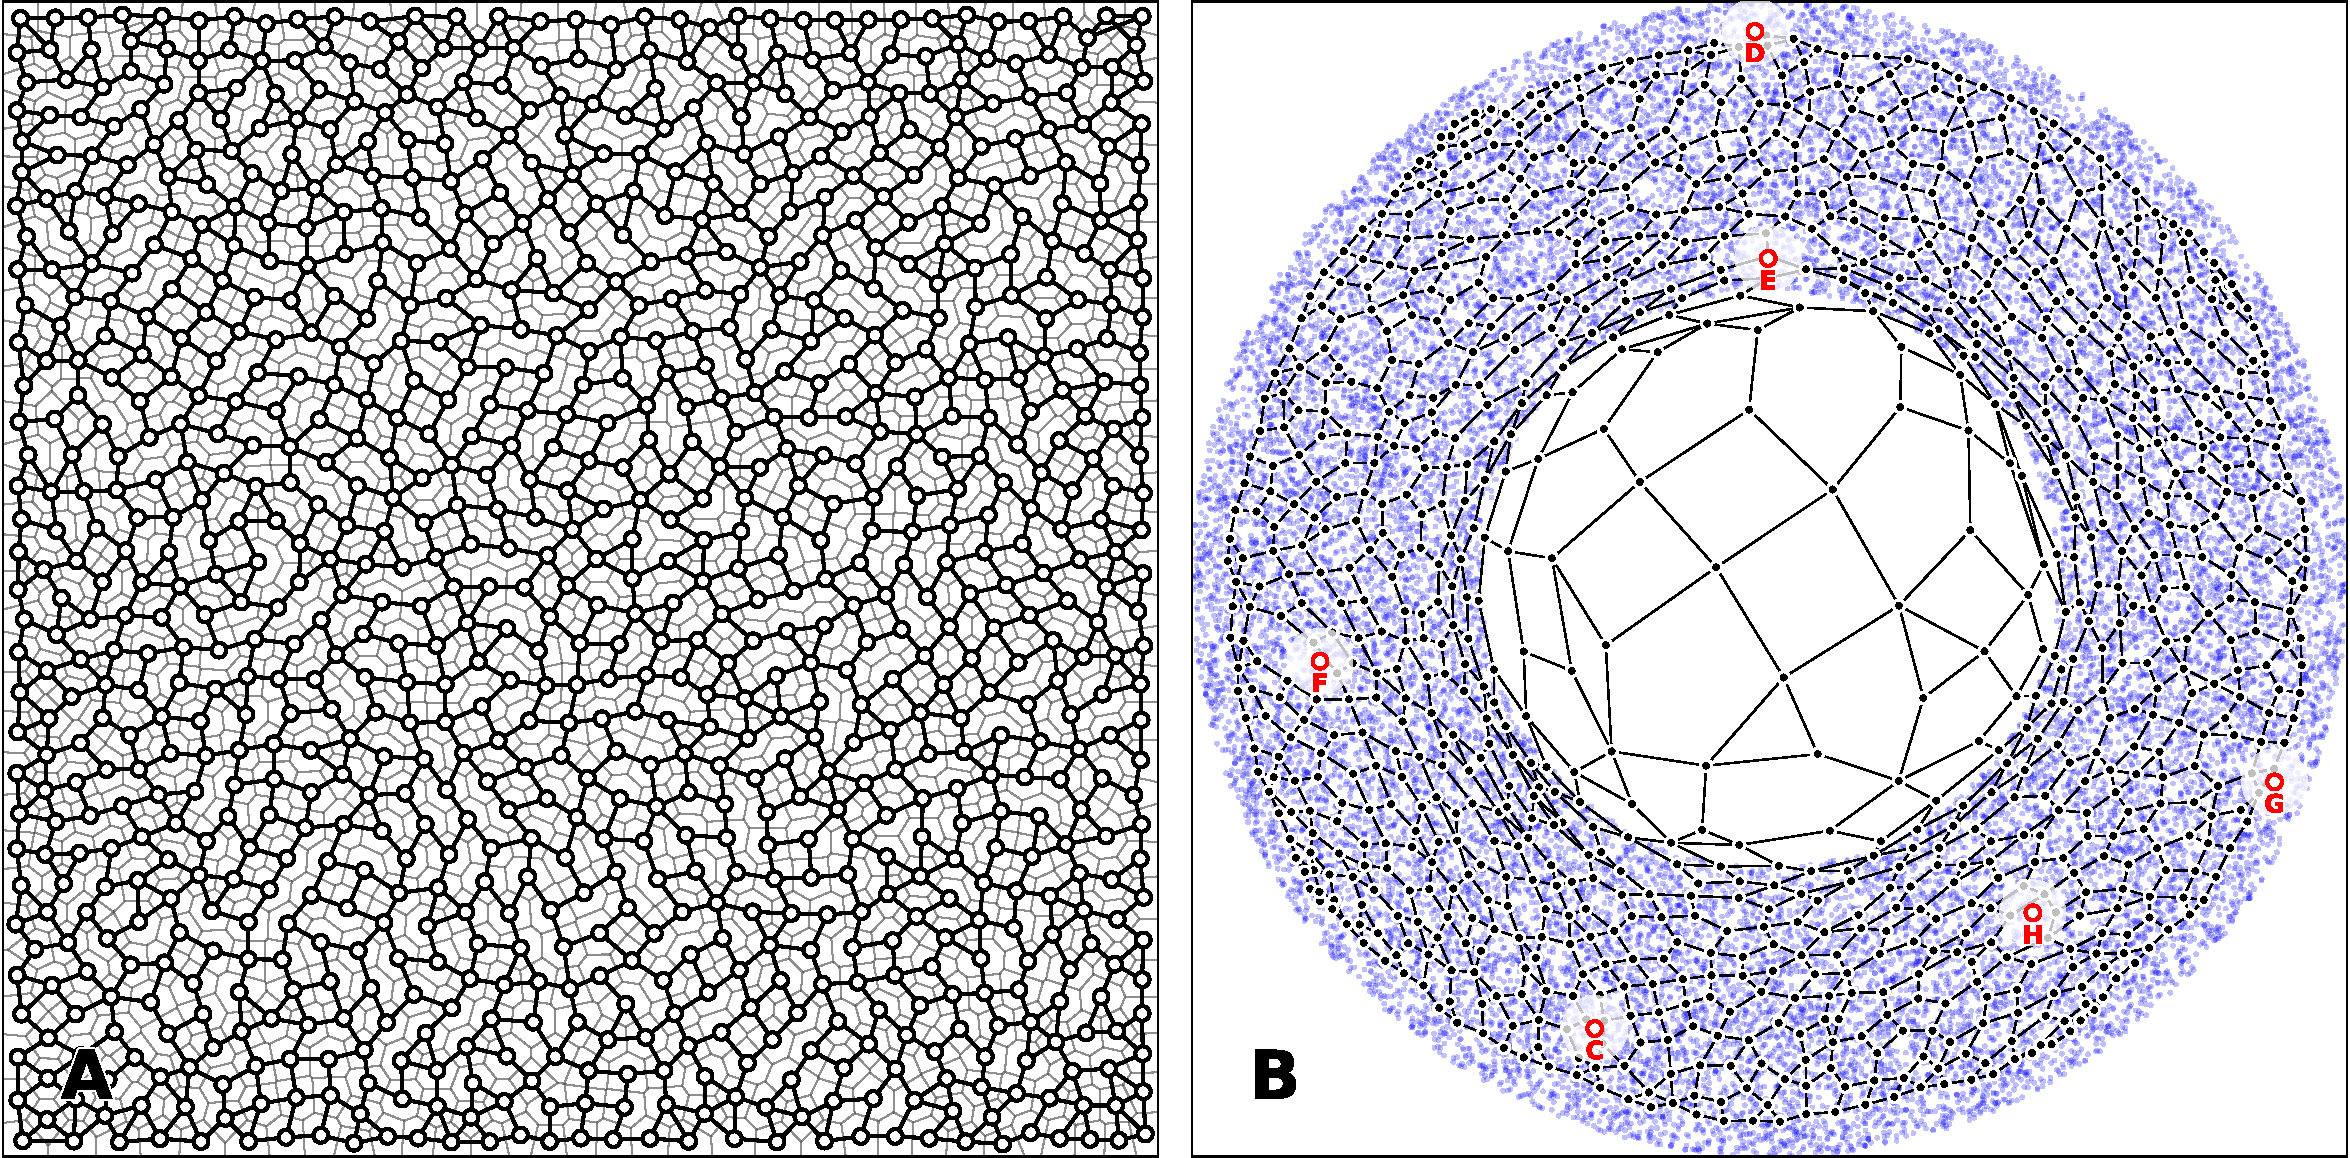
\includegraphics[width=\columnwidth]{figures/vsom-spatial-1.pdf}

  \vspace{2mm}
  
  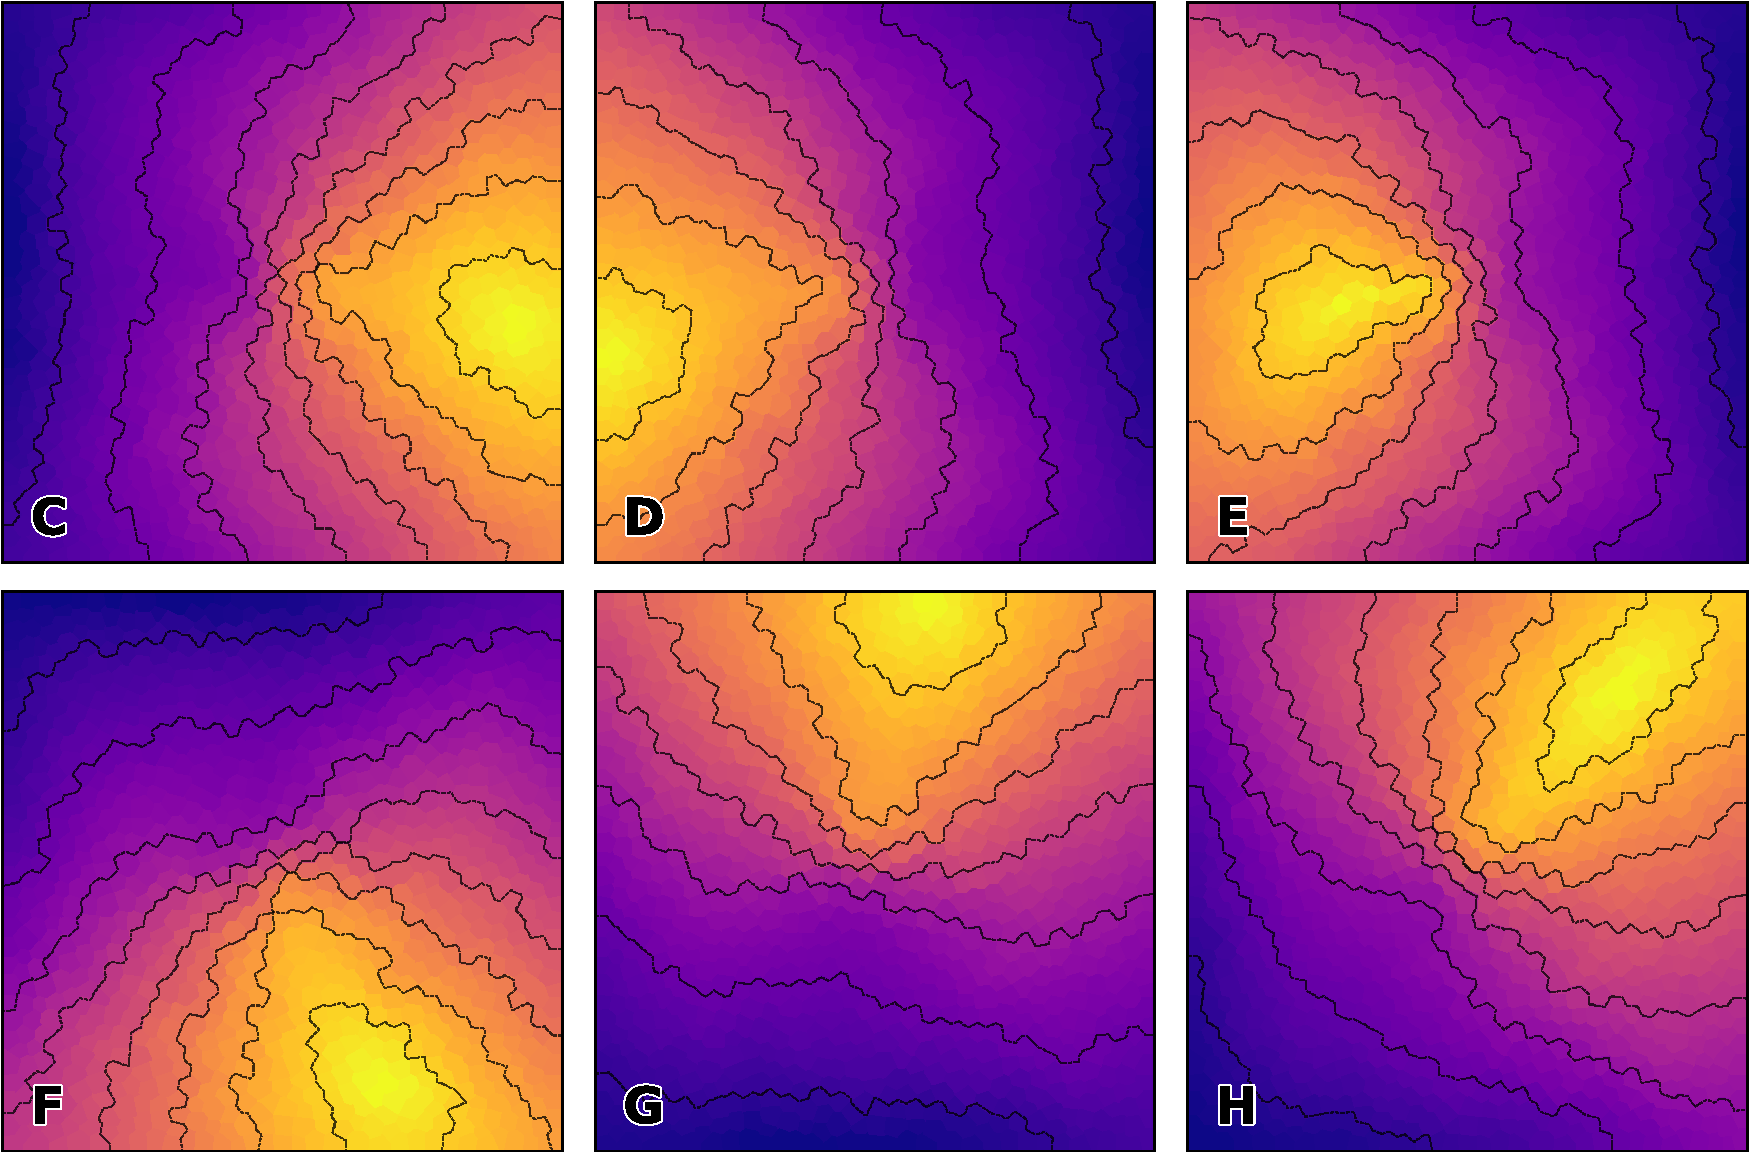
\includegraphics[width=\columnwidth]{figures/vsom-spatial-2.pdf}

  \vspace{2mm}

  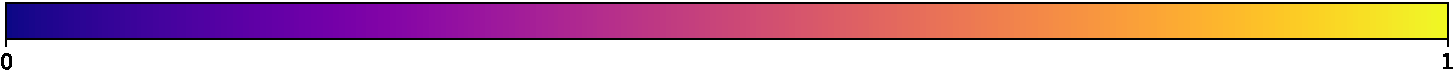
\includegraphics[width=\columnwidth]{figures/colormap.pdf}
  \caption{Voronoidal SOM made of 1003 neurons with a 3-nearest neighbors
    induced topology. Model has been trained for 25,000 epochs on random
    samples inside a torus. \textbf{A} Map topology in the neural
    space. \textbf{B} Map prototypes displayed in data space, blue points are
    the actual samples. \textbf{C to H} Map activity for some random data
    (shown on subplot \textbf{B}).}
\end{figure}

\begin{figure}
  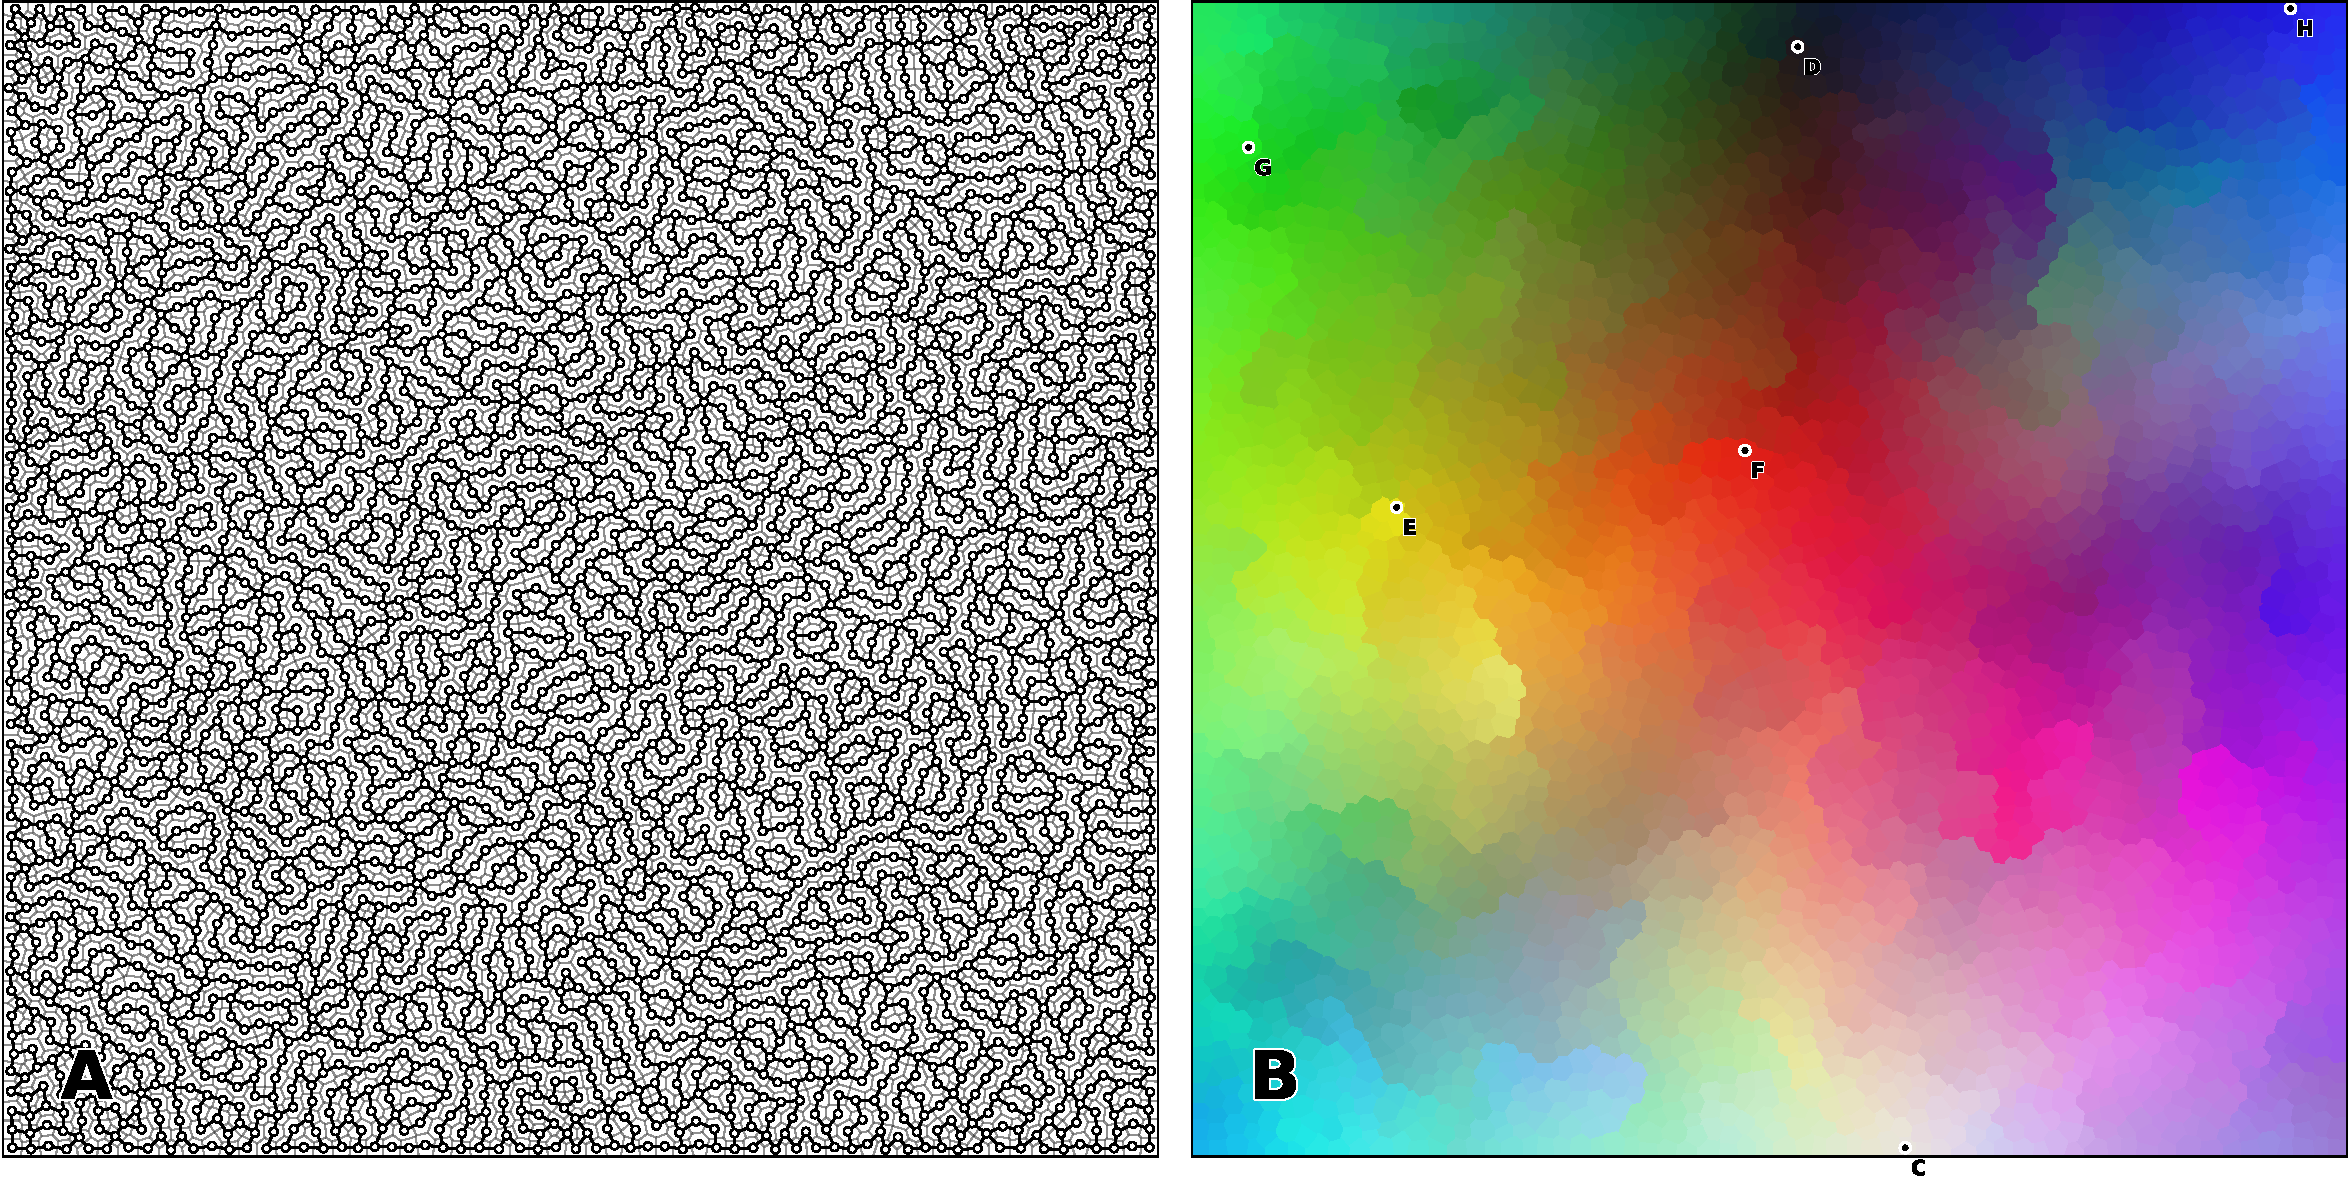
\includegraphics[width=\columnwidth]{figures/vsom-colors-1.pdf}

  \vspace{2mm}
  
  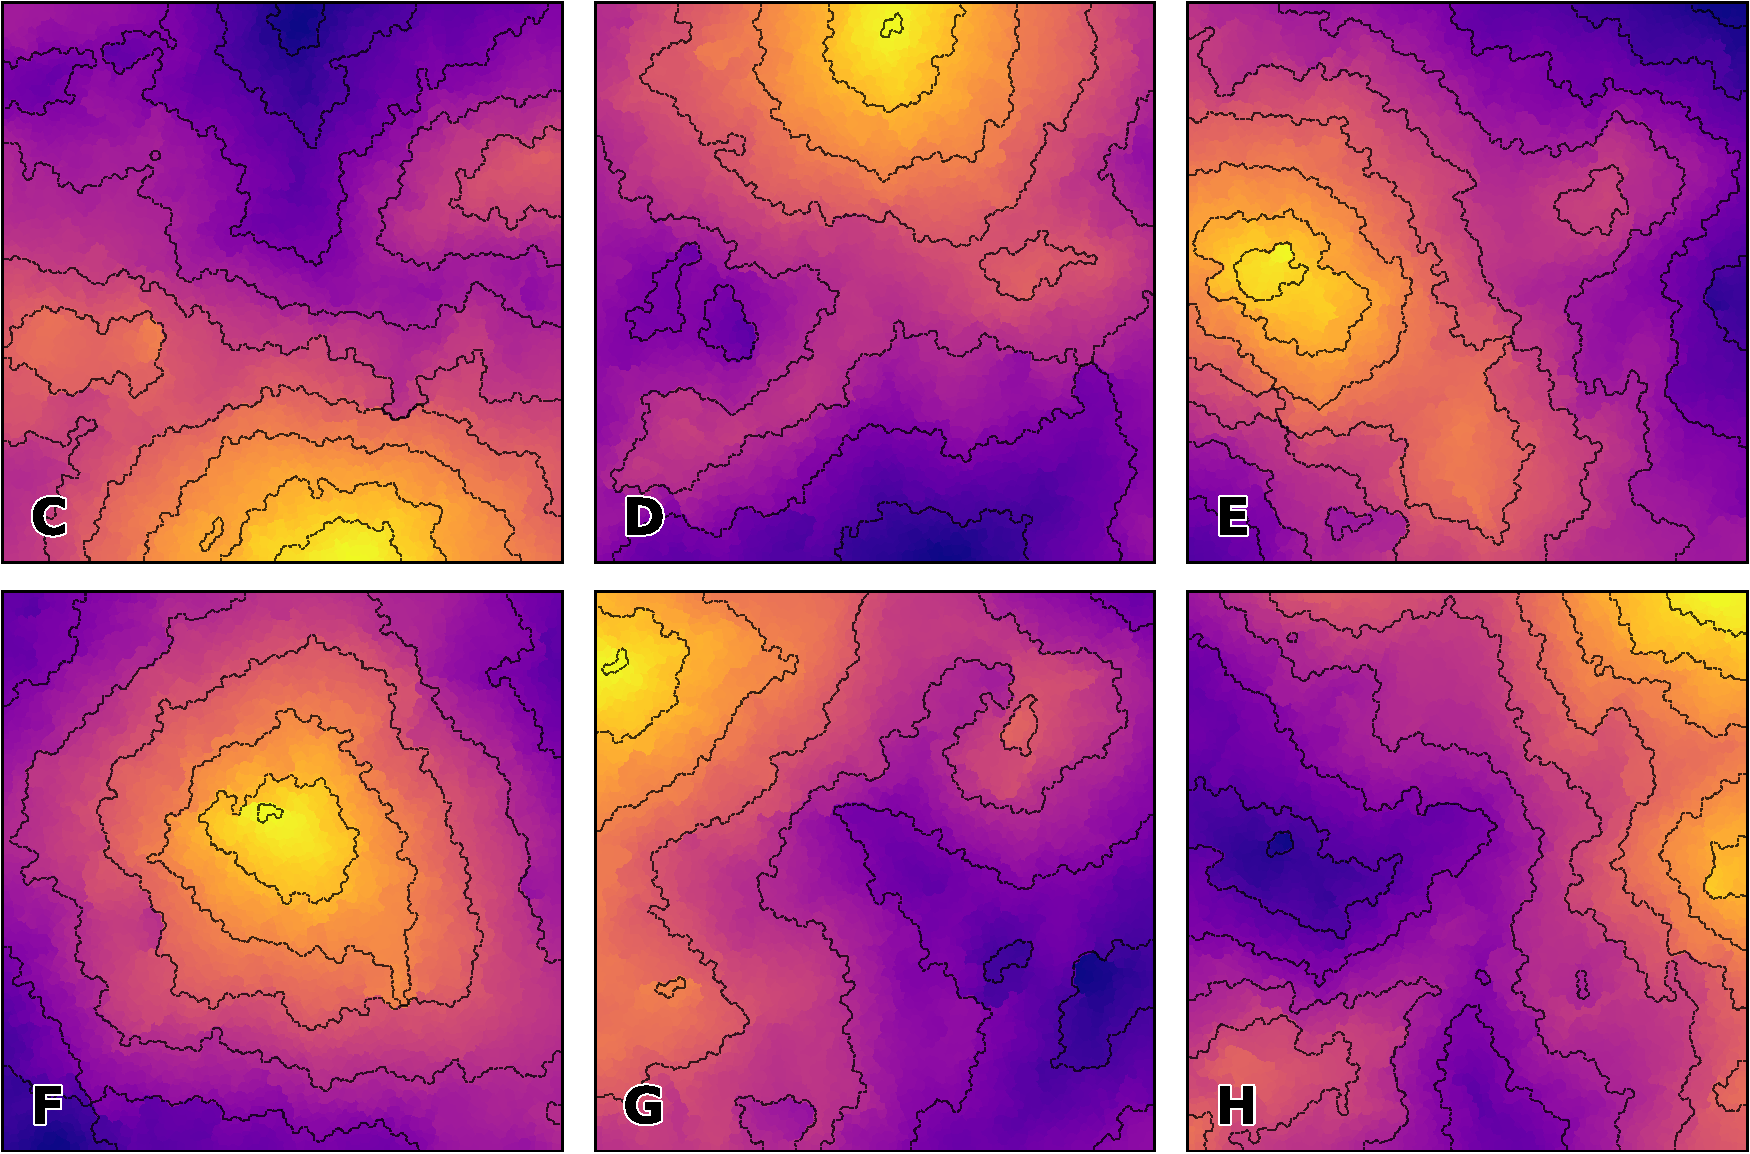
\includegraphics[width=\columnwidth]{figures/vsom-colors-2.pdf}

  \vspace{2mm}

  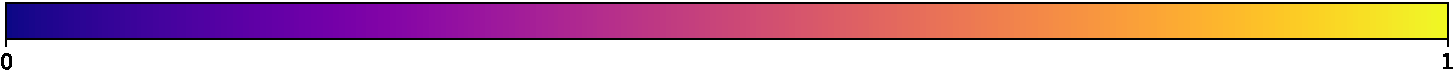
\includegraphics[width=\columnwidth]{figures/colormap.pdf}

  \caption{}
\end{figure}

\subsection{High-dimensional data}






\begin{figure}
  \setlength{\fboxsep}{0pt}%
  \setlength{\fboxrule}{.25pt}%

  \fbox{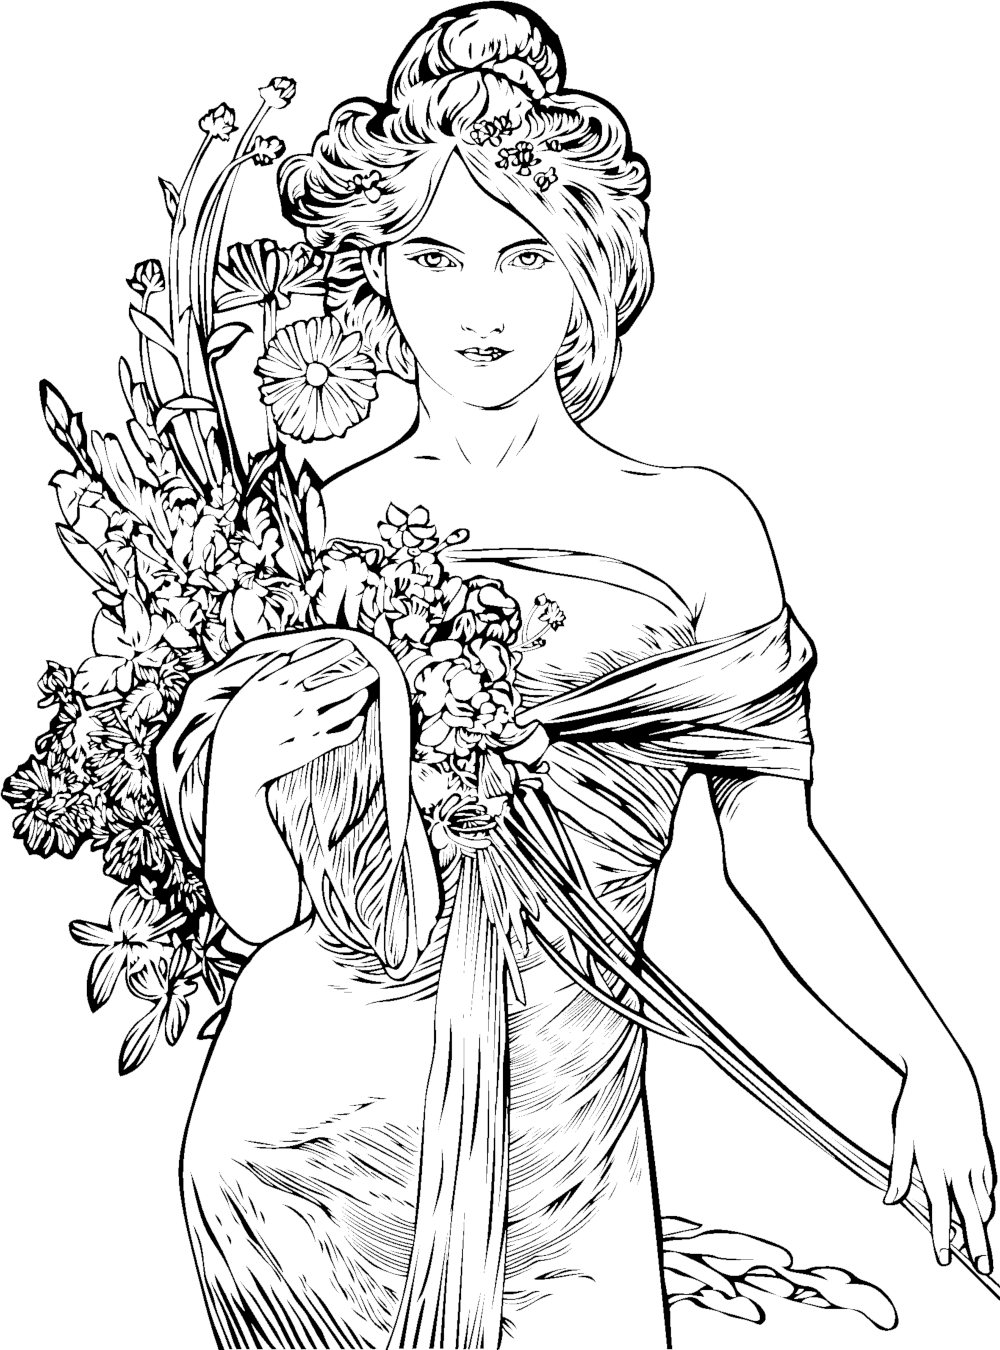
\includegraphics[height=5.1cm]{figures/mucha.png}}
        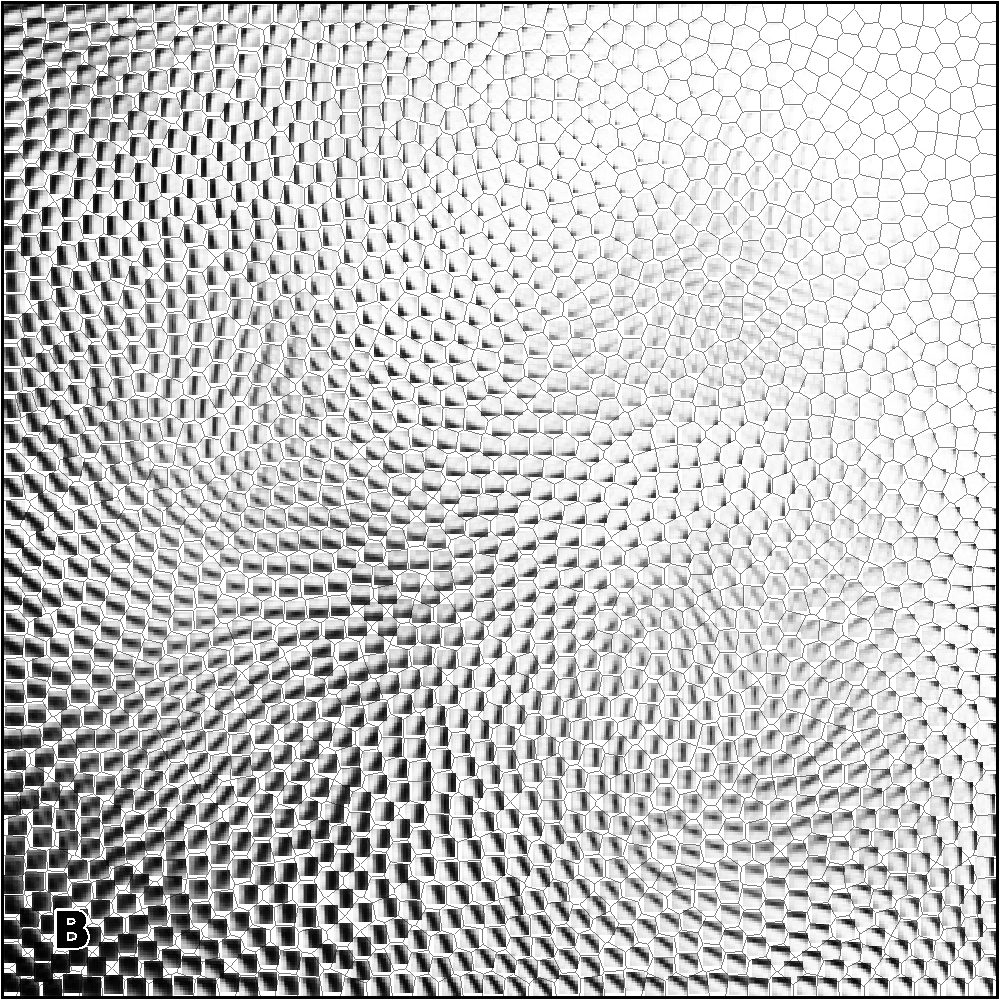
\includegraphics[height=5.1cm]{figures/vsom-image.pdf}
  \fbox{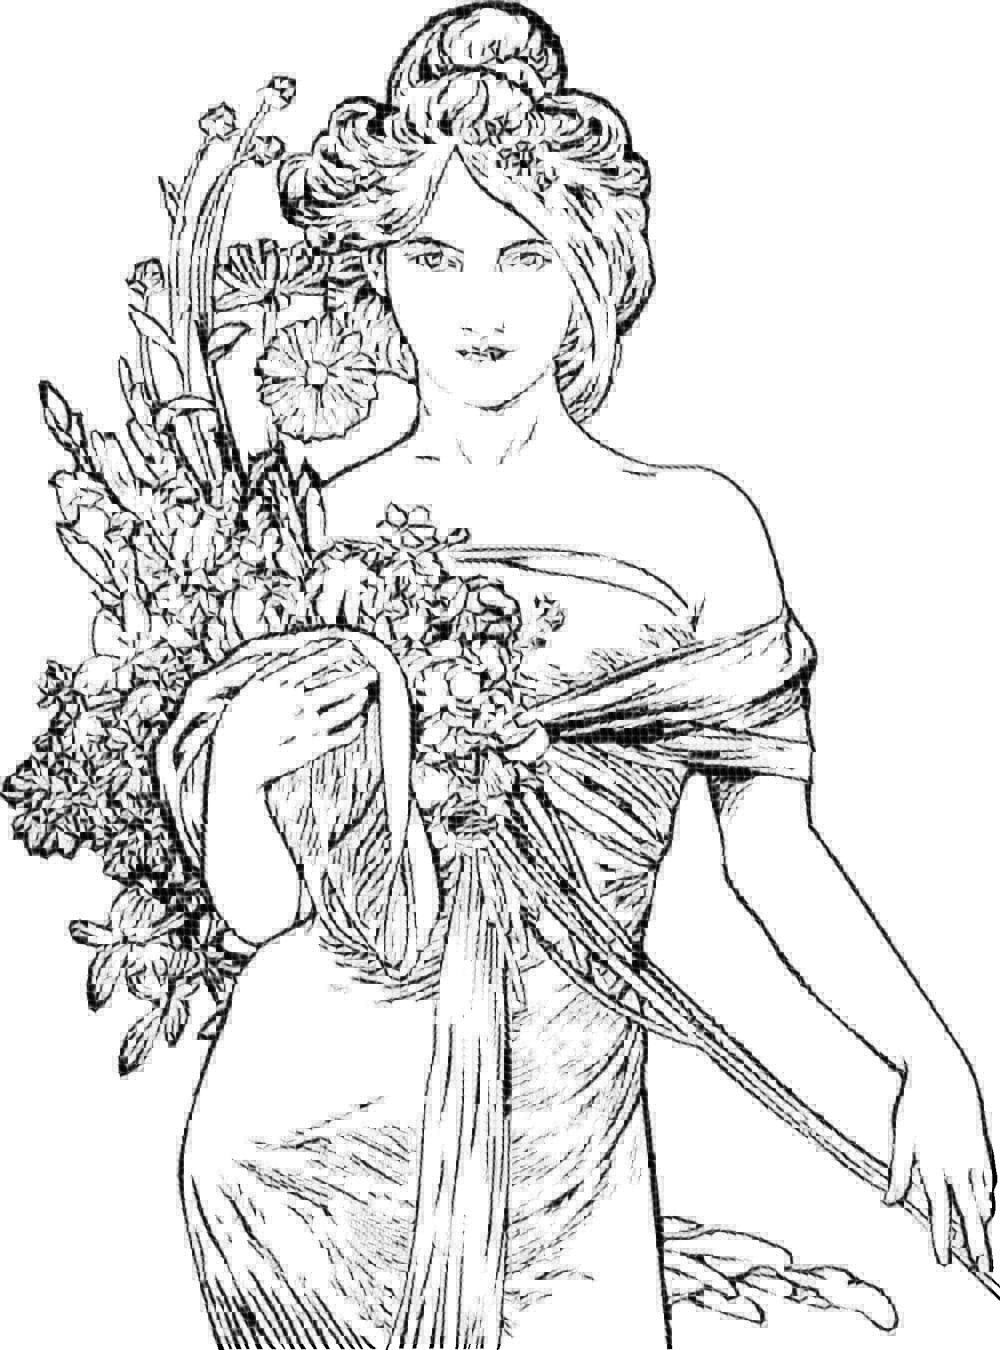
\includegraphics[height=5.1cm]{figures/mucha-vsom.png}}

%  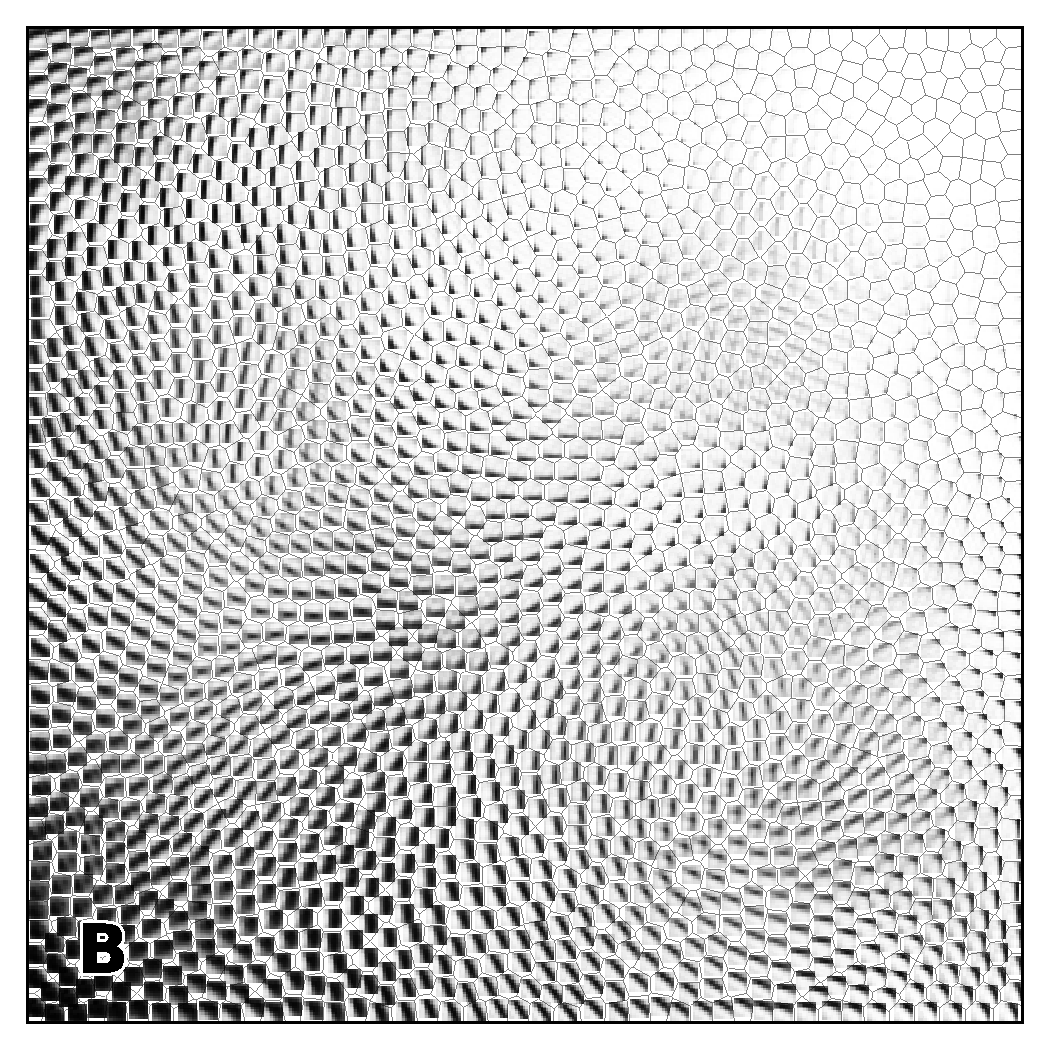
\includegraphics[width=\textwidth]{figures/vsom-image-1.pdf}
  
  \vspace{2mm}

  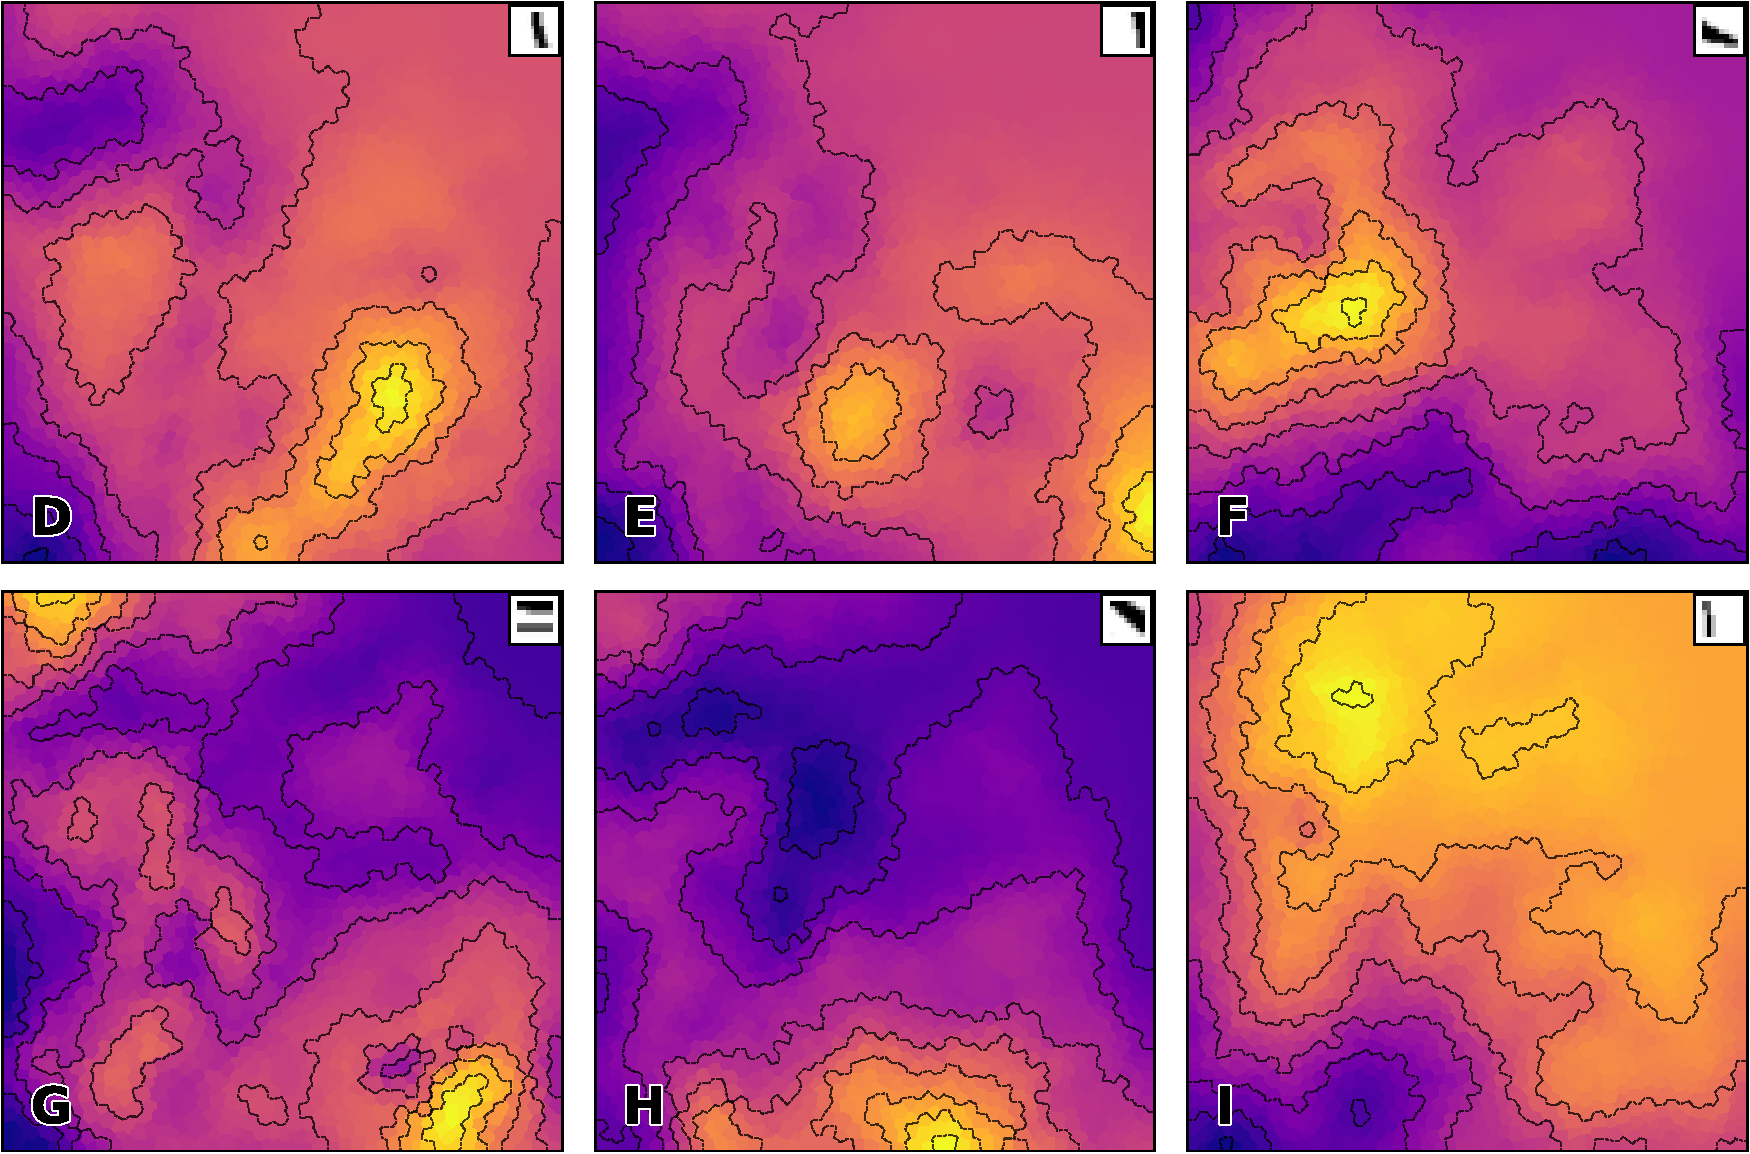
\includegraphics[width=\textwidth]{figures/vsom-image-2.pdf}

  \caption{Voronoidal SOM made of 1003 neurons with a 2-nearest neighbors
    induced topology. Model has been trained for 10,000 epochs on random
    uniform scalars in [0,1]. \textbf{A} Map topology in the neural
    space. \textbf{B} Map prototypes displayed in neural space using Voronoi
    cells (whose color indicates prototype according to colormap). \textbf{C to
      H} Map activity for some random data (\textbf{C}:0.0, \textbf{D}:0.2,
    \textbf{E}: 0.4, \textbf{F}:0.6, \textbf{G}:0.8, \textbf{H}:1.0).}
\end{figure}


\subsection{Reorganization}

In case of neural loss (a set of neurons is removed from the map) or neural
gain (a set of neurons is added to the map), we can appy the LLoyd relaxation
scheme in order to achieve a new quasi centroidal Voronoi tesselation (see
figure \ref{fig:CVT}) whose induced topology shares similarity with the orginal
topology (before loss or gain).

\begin{figure}
  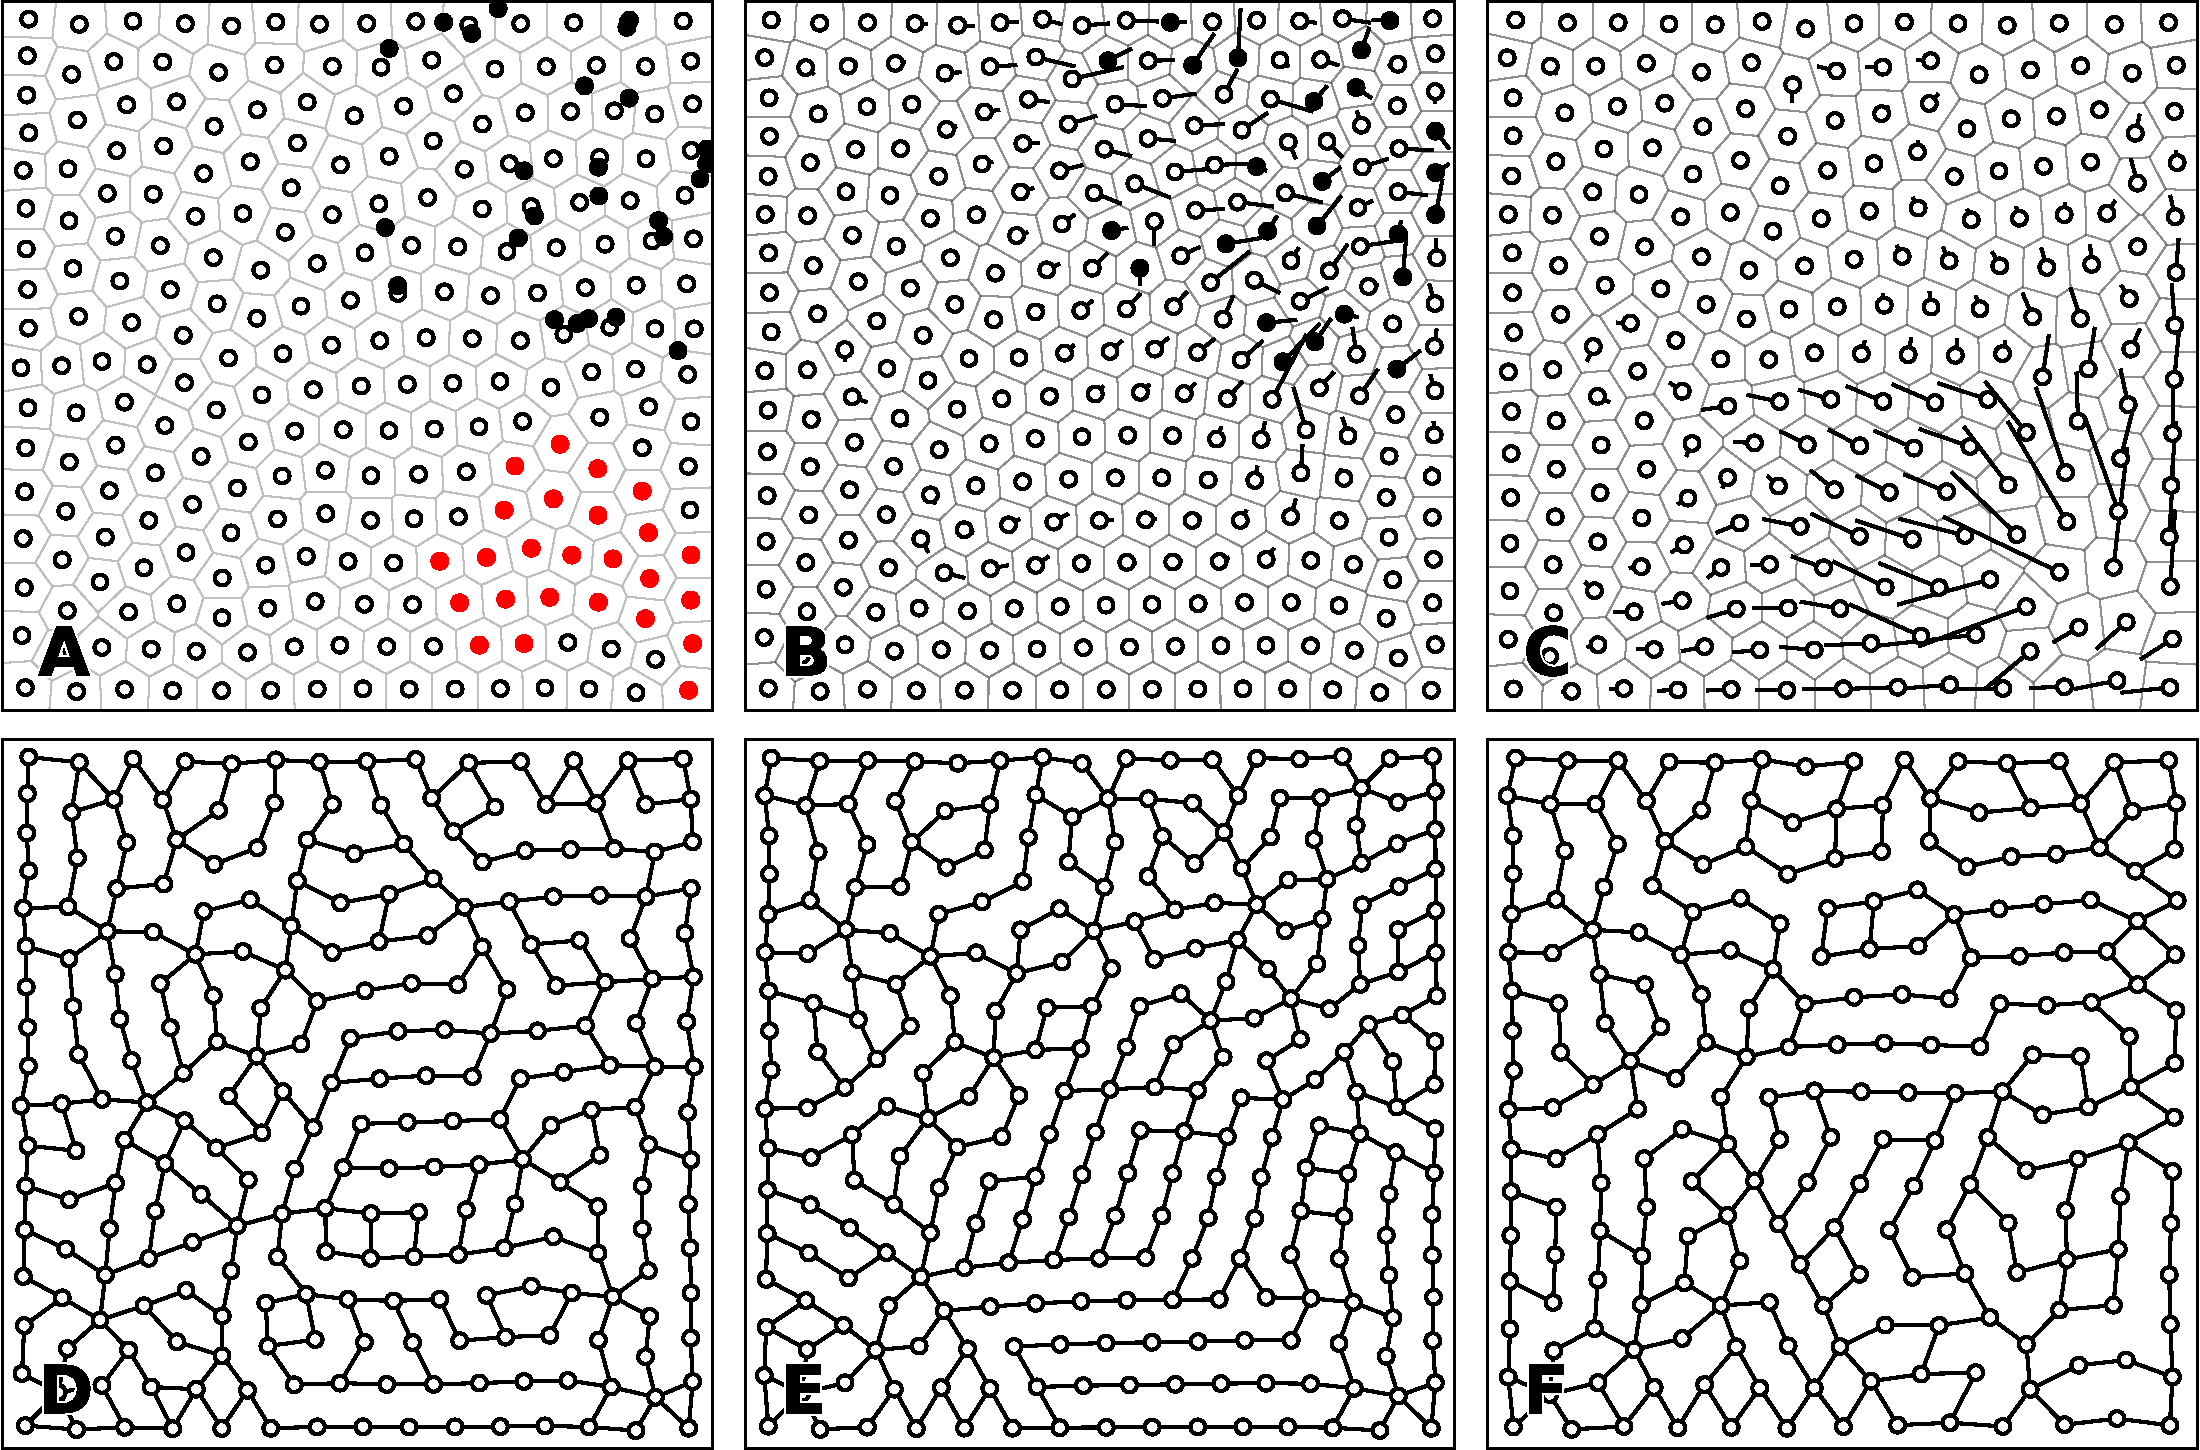
\includegraphics[width=\columnwidth]{figures/vsom-resilience.pdf}
  \caption{\textbf{Reorganization following neural loss or gain.}  An initial
    set of 248 neurons (outlined discs on panel \textbf{A}) has been modified
    with the addition of 25 neurons (black discs) or the removal of 25 neurons
    (red discs). Panels \textbf{B} and \textbf{C} show the final position of
    neurons after 100 iterations of the centroidal Voronoi tesselation. Lines
    shows individual movement of neurons. Panels \textbf{D}, \textbf{E} and
    \textbf{F} show the 2-neighbors induced topology for \textbf{A},
    \textbf{B} and \textbf{C} respectively.}
  \label{fig:CVT}
\end{figure}

\subsubsection*{Ablation}

\subsubsection*{Addition}
